\begin{centering}

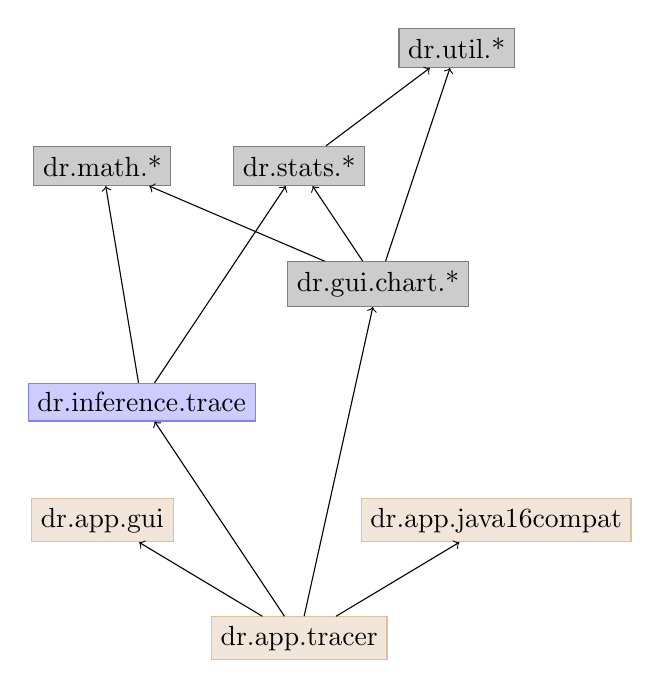
\begin{tikzpicture}[rectangle, package/.style={draw=black!50,fill=black!20}, infpackage/.style={draw=blue!50,fill=blue!20}, evopackage/.style={draw=green!50,fill=green!20}, apppackage/.style={draw=brown!50,fill=brown!20}]

\node[apppackage] (appgui) at (-2.5, -1.5) {dr.app.gui}; 
\node[apppackage] (appjava) at (2.5, -1.5) {dr.app.java16compat}; 
\node[apppackage] (tracer) at (0, -3) {dr.app.tracer}; 
\node[infpackage] (inference) at (-2, 0) {dr.inference.trace}; 
\node[package] (stats) at (0, 3) {dr.stats.*}; 
\node[package] (util) at (2, 4.5) {dr.util.*}; 
\node[package] (math) at (-2.5, 3) {dr.math.*}; 
\node[package] (gui) at (1, 1.5) {dr.gui.chart.*}; 

\draw [->] (gui) -- (util); 
\draw [->] (gui) -- (stats); 
\draw [->] (gui) -- (math); 
\draw [->] (tracer) -- (gui); 
\draw [->] (tracer) -- (appgui); 
\draw [->] (tracer) -- (appjava); 
\draw [->] (tracer) -- (inference); 
\draw [->] (inference) -- (math); 
\draw [->] (inference) -- (stats); 
\draw [->] (stats) -- (util); 

\end{tikzpicture} 

\end{centering}